\documentclass[10pt]{article} 

\usepackage{amsmath,amssymb,amsthm,amsfonts} % assumes amsmath package installed
\usepackage[linktocpage=true,colorlinks=true,linkcolor=blue,citecolor=blue,urlcolor=blue]{hyperref}
\usepackage[letterpaper,margin=0.9in]{geometry}

% \newtheorem{definition}{Definition}
% \newtheorem{assumption}{Assumption}
% \newtheorem{theorem}{Theorem}
% \newtheorem{conjecture}{Conjecture}
% \newtheorem{lemma}{Lemma}
% \newtheorem{proposition}{Proposition}
% \newtheorem{remark}{Remark}

\newcommand{\bx}{\boldsymbol{x}}
\newcommand{\be}{\boldsymbol{e}}
\newcommand{\blambda}{\boldsymbol{\lambda}}
\newcommand{\bLambda}{\boldsymbol{\Lambda}}
\newcommand{\bu}{\boldsymbol{u}}
\newcommand{\bw}{\boldsymbol{w}}
\newcommand{\by}{\boldsymbol{y}}
\newcommand{\bz}{\boldsymbol{z}}
\newcommand{\bV}{\boldsymbol{V}}
\newcommand{\bX}{\boldsymbol{X}}
\newcommand{\bY}{\boldsymbol{Y}}
\newcommand{\bZ}{\boldsymbol{Z}}
\newcommand{\bv}{\boldsymbol{v}}
\newcommand{\bxi}{\boldsymbol{\xi}}
\newcommand{\bpi}{\boldsymbol{\pi}}
\newcommand{\bphi}{\boldsymbol{\phi}}
\newcommand{\bbeta}{\boldsymbol{\eta}}
\newcommand{\bpsi}{\boldsymbol{\psi}}
\newcommand{\bzeta}{\boldsymbol{\zeta}}
\newcommand{\bmu}{\boldsymbol{\mu}}
\newcommand{\bq}{\boldsymbol{q}}
\newcommand{\bQ}{\boldsymbol{Q}}
\newcommand{\bK}{\boldsymbol{K}}
\newcommand{\bP}{\boldsymbol{P}}
\newcommand{\bS}{\boldsymbol{S}}
\newcommand{\bT}{\boldsymbol{T}}
\newcommand{\bF}{\boldsymbol{F}}
\newcommand{\bG}{\boldsymbol{G}}
\newcommand{\bd}{\boldsymbol{d}}
\newcommand{\bp}{\boldsymbol{p}}
\newcommand{\bff}{\boldsymbol{f}}
\newcommand{\bc}{\boldsymbol{c}}
\newcommand{\bg}{\boldsymbol{g}}
\newcommand{\bh}{\boldsymbol{h}}
\newcommand{\bA}{\boldsymbol{A}}
\newcommand{\bL}{\boldsymbol{L}}
\newcommand{\ba}{\boldsymbol{a}}
\newcommand{\bb}{\boldsymbol{b}}
\newcommand{\bB}{\boldsymbol{B}}
\newcommand{\bC}{\boldsymbol{C}}
\newcommand{\bE}{\boldsymbol{E}}
\newcommand{\bH}{\boldsymbol{H}}
\newcommand{\bR}{\boldsymbol{R}}
\newcommand{\bn}{\boldsymbol{n}}
\newcommand{\bm}{\boldsymbol{m}}
\newcommand{\br}{\boldsymbol{r}}
\newcommand{\bl}{\boldsymbol{l}}
\newcommand{\bI}{\boldsymbol{I}}
\newcommand{\osigma}{\overline{\sigma}}
\newcommand{\usigma}{\underline{\sigma}}
\newcommand{\oosigma}{\overline{\osigma}}
\newcommand{\uusigma}{\underline{\usigma}}
\newcommand{\olambda}{\overline{\lambda}}
\newcommand{\ulambda}{\underline{\lambda}}
\newcommand{\oolambda}{\overline{\olambda}}
\newcommand{\uulambda}{\underline{\ulambda}}
\newcommand{\bzero}{\boldsymbol{0}}
\newcommand{\dist}{\text{\normalfont dist}}
\newcommand{\st}{\mathop{\text{\normalfont s.t.}}}
\newcommand{\diag}{\mathop{\text{\normalfont diag}}}
\newcommand{\amin}{\mathop{\text{\normalfont argmin}}}
\newcommand{\ReH}{\mathop{\text{\normalfont ReH}}}
\newcommand{\bbZ}{\mathbb{Z}}
\newcommand{\cG}{\mathcal{G}}
\newcommand{\cV}{\mathcal{V}}
\newcommand{\cW}{\mathcal{W}}
\newcommand{\cA}{\mathcal{A}}
\newcommand{\cB}{\mathcal{B}}
\newcommand{\cL}{\mathcal{L}}
\newcommand{\cE}{\mathcal{E}}
\newcommand{\cD}{\mathcal{D}}
\newcommand{\cP}{\mathcal{P}}
\newcommand{\cQ}{\mathcal{Q}}
\newcommand{\cK}{\mathcal{K}}
\newcommand{\cM}{\mathcal{M}}
\newcommand{\cN}{\mathcal{N}}
\newcommand{\cI}{\mathcal{I}}
\newcommand{\cJ}{\mathcal{J}}
\newcommand{\cT}{\mathcal{T}}
\newcommand{\interior}{\mathop{\text{\normalfont interior}}}
\newcommand{\relint}{\mathop{\text{\normalfont relint}}}
\newcommand{\vertices}{\mathop{\text{\normalfont vertices}}} 
\sloppy
\usepackage{graphicx}

\usepackage{enumitem} 
\usepackage{mathtools}
\allowdisplaybreaks
\renewcommand{\theenumi}{(\alph{enumi})} 
\usepackage{parskip}

\usepackage{tikz}

\usepackage{multirow}
\usepackage{pifont}
\newcommand{\cmark}{\ding{51}}%
\newcommand{\xmark}{\ding{55}}%



\title{{\bfseries Sparse Condensed-Space Interior-Point Methods with Inequality Relaxations on GPUs: Will it Work?}}

\graphicspath{}

\author[Sungho Shin]{
  Sungho Shin\\
  {\normalfont\footnotesize\url{sshin@anl.gov}}
}
\subtitle{}
\institute[ANL/MCS]{
  Argonne National Laboratory
}

\begin{document}

{
  % \usebackgroundtemplate{\includegraphics[width=\paperwidth]{TitleANLBlue}}
  \frame[noframenumbering,plain]{
    \titlepage
    \vspace{-.7in}
  }
}

\begin{frame}{Executive Summary}
  \begin{itemize}
  \item We exmaine the potential benefit of sparse condensed-space interior-point methods with inequality relaxations, with the goal of solving general large-scale NLPs on GPUs.
  \item The proposed method relaxes the equality constraints as inequality constraints by replacing $c(x) =0$ by $c(x)+ s=0$ and $0\leq s\leq\epsilon_{\text{IR}}$.
  \item The resulting inequality-constrained NLP is solved with sparse condensed-space interior-point method, which requires solving a sparse positive definite system.
  \item While the LU solver in CUSOLVERRF cannot handle the sparse indefinite systems wihtin IPM, it can handle the sparse PD systems up to a certain accuracy ($\epsilon_{\text{IR}}=\texttt{tol} = 10^{-3}$).
  \item For portability, we will still need a sparse Cholesky solver running on GPU.
  \end{itemize}
\end{frame}

\begin{frame}{A Naive Approach Doesn't Work.}
  \begin{itemize}
  \item Can we solve the indefinite KKT systems using sparse LU solver in \texttt{CUSOLVERRF}? No.
    \begin{center}
      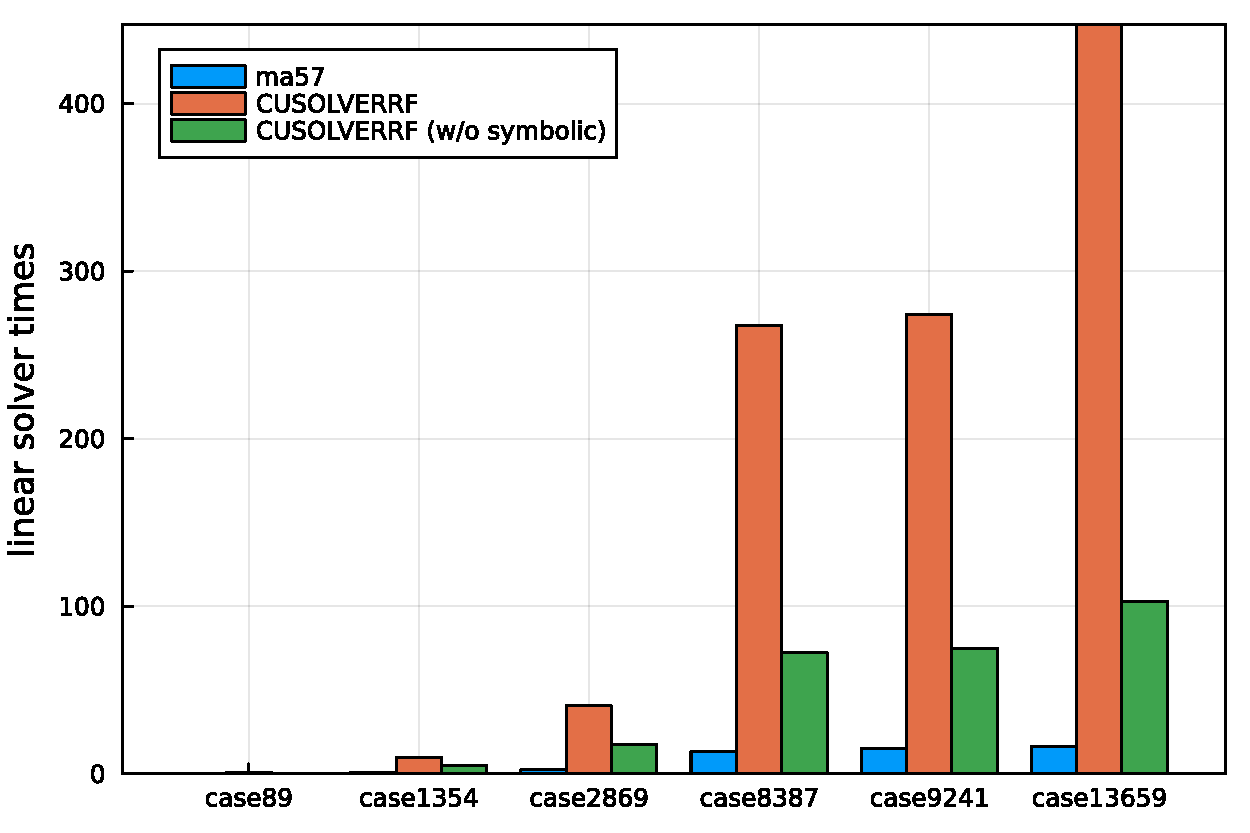
\includegraphics[width=.5\textwidth]{../fig/linear_solvers.pdf}  
    \end{center}   
  \item Symbolic factorization needed every several iterations (every 3 for above case).
  \item Numeric factorization is not fast.
  \end{itemize}  
\end{frame}

\begin{frame}{Condensed Approach}
  Consider an NLP of the following form: 
  \begin{align*}
    \mathop{\text{min}}_{x^L\leq x\leq x^U}\;& f(x)\;\\
    \st\;&c(x) = 0.
  \end{align*}
  The problem is relaxed via {\it inequality relaxation}:
  \begin{align*}
    \mathop{\text{min}}_{x^L\leq x\leq x^U, 0\leq s \leq \epsilon_{\text{IR}}}\;& f(x)\;\\
    \st\;& c(x) + s= 0,
  \end{align*}
  where $\epsilon_{\text{IR}}\approx\texttt{tol}$.

  We now observe that the problem has {\it inequality constriants only}. This allows us to apply the {\it condensation strategy}:
  \begin{align*}
    \begin{bmatrix}
      H + \Sigma_x & &J^\top \\
      & \Sigma_s &I \\
      J & I &\\
    \end{bmatrix}
    \begin{bmatrix}
      p^u \\ p^s \\ p^\lambda
    \end{bmatrix}  = -
    \begin{bmatrix}
      r_1 \\ r_2 \\ r_3 ,
    \end{bmatrix}
    \iff \left(H + \Sigma_x+ J^\top \Sigma_s J \right) p^u = -r_1 + J r_2 - J^\top \Sigma_s r_3.
  \end{align*}
  Of course, $J^\top \Sigma_s J$ can be arbitrarily dense, but our favorite problems (e.g., OPF) will still be sparse.
\end{frame}

\begin{frame}{Effects of Inequality Relaxation}
  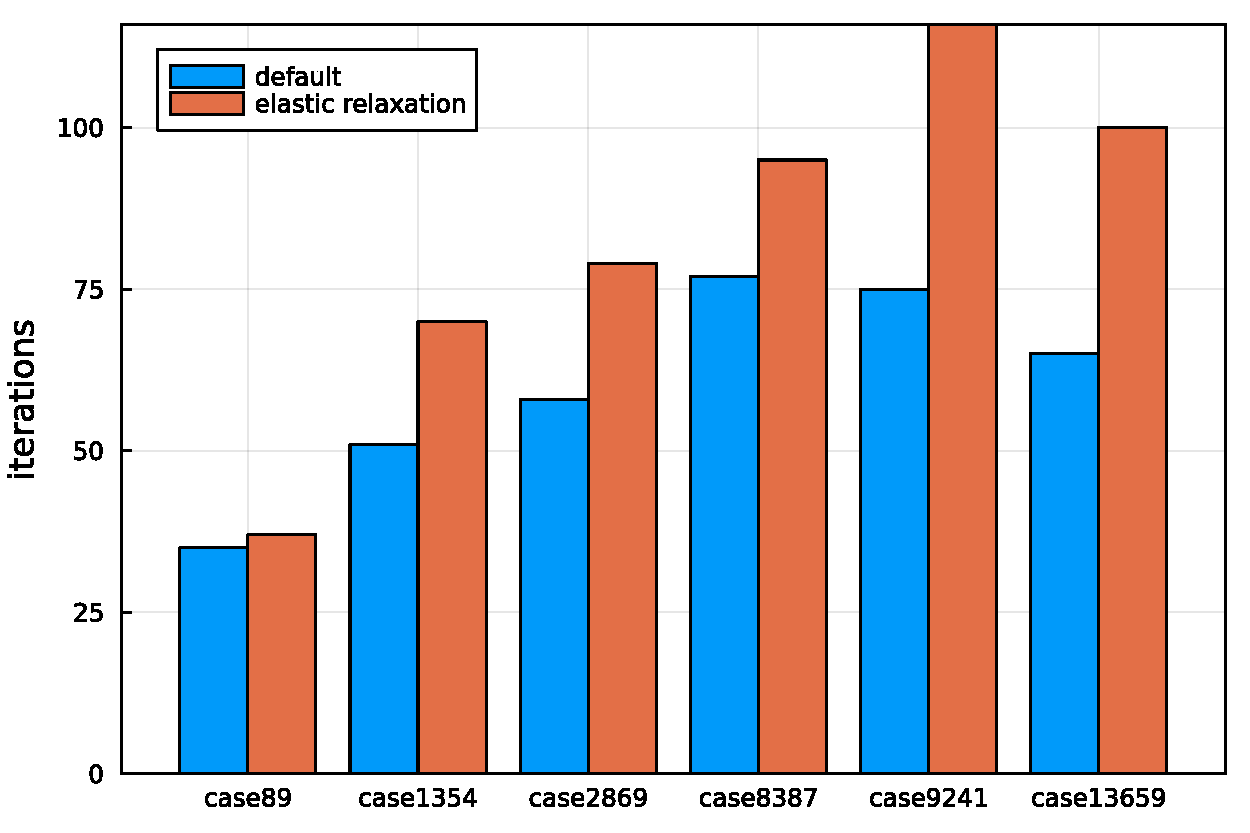
\includegraphics[width=.32\textwidth]{../fig/iter.pdf}
  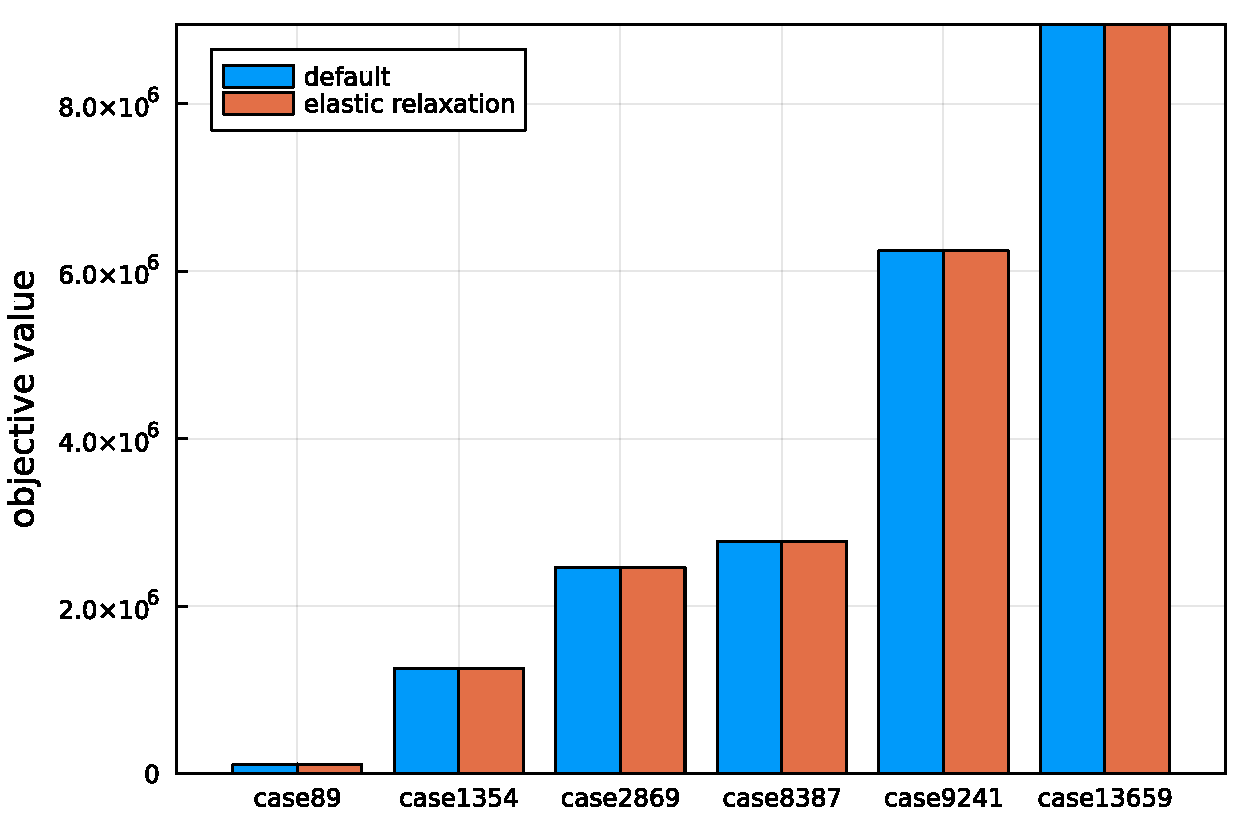
\includegraphics[width=.32\textwidth]{../fig/objval.pdf}
  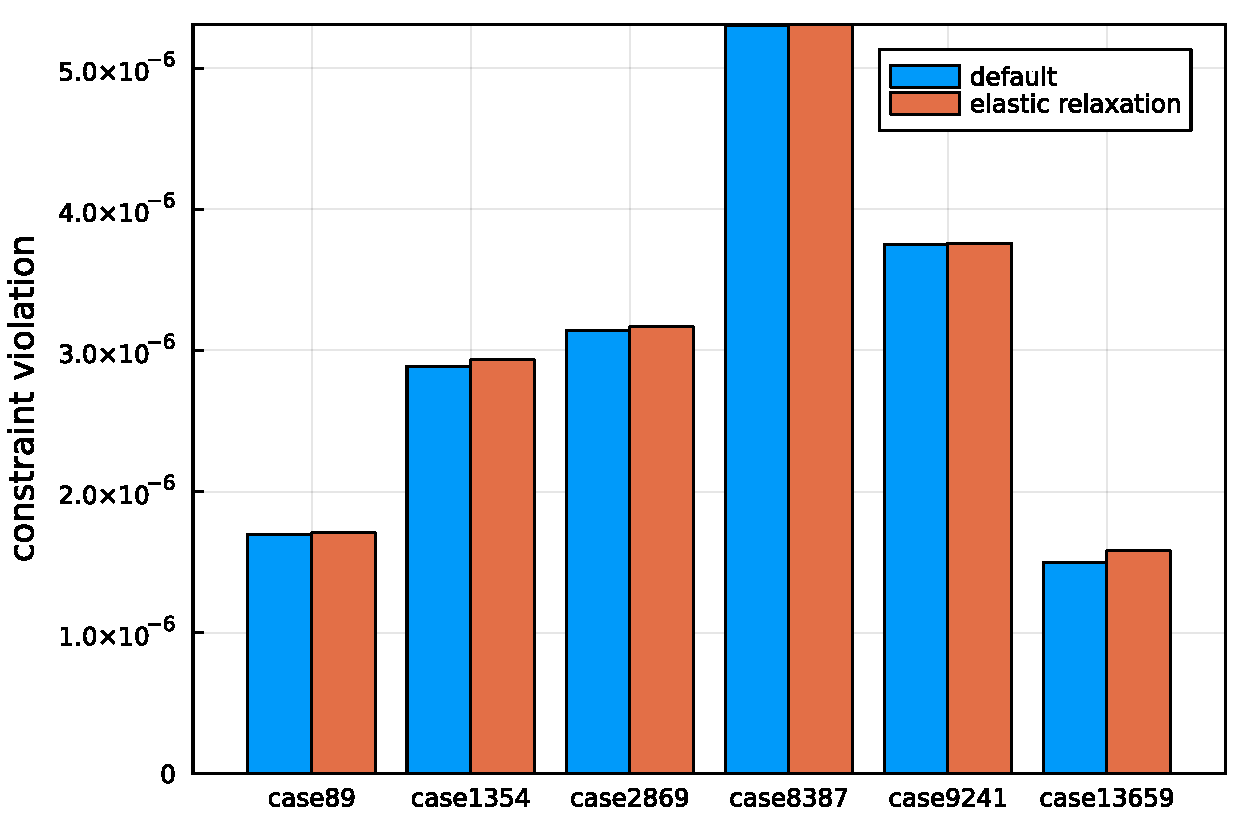
\includegraphics[width=.32\textwidth]{../fig/cvio.pdf}
  \begin{itemize}
  \item $\epsilon_{\text{IR}}=10^{-8}$
  \item Number of iterations increased (5--50\%).
  \item Not much difference in the quality of solution (obj value/constraint violation).
  \end{itemize}
\end{frame}

\begin{frame}{Will it be Efficient?}
  \begin{itemize}
  \item We do this experiment to better evaluate the potential benefit of the proposed strategy.
  \item We take the KKT system from the iterates obtained from MadNLP+Ma57 and solve it with CUSOLVER. We aim to check:
    \begin{itemize}
    \item Symbolic factorization can be reused between iterations.
    \item Numeric factorization/backsolve is fast/precise enough. 
    \end{itemize}
    \begin{center}
      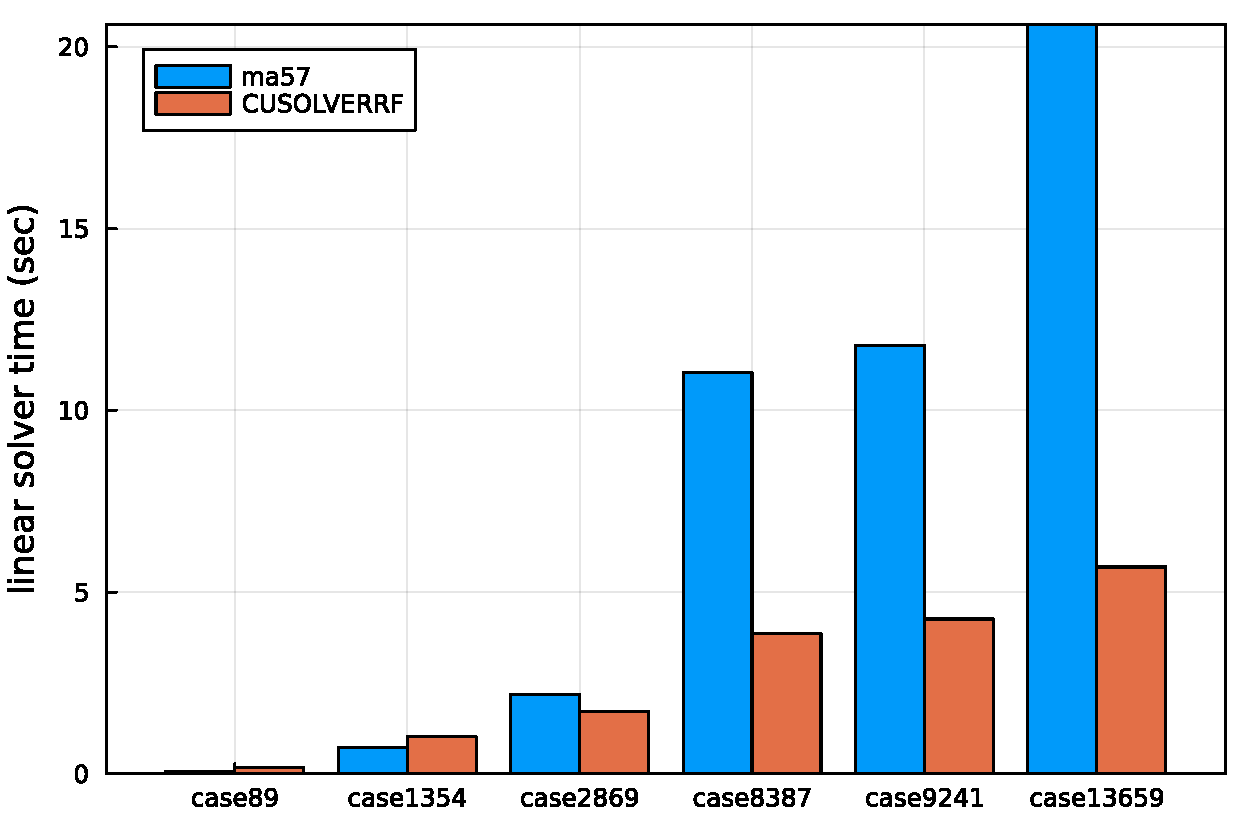
\includegraphics[width=.5\textwidth]{../fig/hypo.pdf}  
    \end{center}
  \item Observation: factorization/backsolve is precise/efficient enough for $\epsilon_{\text{IR}}=\texttt{tol} = 10^{-3}$.
  \end{itemize}
\end{frame}

\begin{frame}{What do we need for Portabiltiy?}
  \begin{itemize}
  \item For now, the sparse LU solver in CUSOLVERRF can do the job.
  \item For portability, all we need is a sparse Cholesky solver (preferrably, written in {\tt KernelAbstractions.jl}).
  \end{itemize}
\end{frame}

% \begin{frame}{Schur Complement as ``Bandwidth Thickening''}
%   \begin{itemize}
%   \item Directly solving large-scale 
%   \item Can be applied to any graph-structured sparse systems.
%   \end{itemize}
% \end{frame}

% \def\checkmark{$\text{\rlap{$\checkmark$}}\square$} 
\begin{frame}{Current Status (6/27/2023)}
  \begin{itemize}
  \item SparseCondensedKKTSystem works on CPU.
  \item With inequality relaxation, can solve {\tt case9241} up to ${\tt tol} = 10^{-7}$, but requires long iterative refinement. Convergence up to $10^{-5}$ is reliable/efficient.
  \item Numerical results (w/ linear algebra/AD on GPU) for {\tt case9241}:
    \begin{center}
      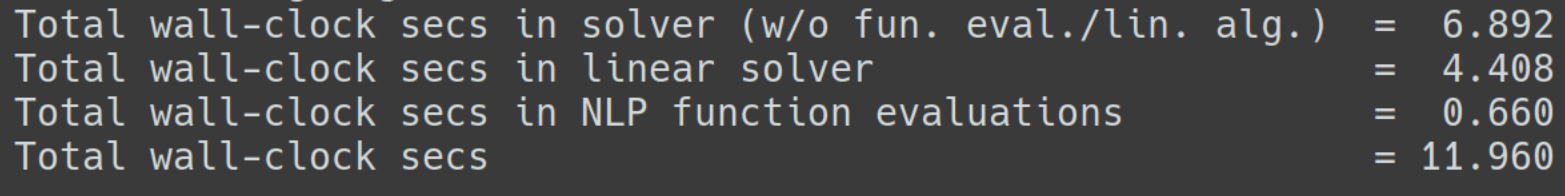
\includegraphics[width=.8\textwidth]{../fig/result-6-27.png}
    \end{center}
    \begin{itemize}
    \item Linear Sovler: only 0.708 secs out of 4.408 secs are spent on GPU.
    \item AD: only 0.104 secs out of 0.660 secs are spent on GPU.
    \item MadNLP: operations like $y \leftarrow y + ax$ are $\times 10$ faster on GPUs.
    \end{itemize}  
  \item By running everything on GPUs, we may solve {\tt case9241} in less than 4 secs (JuMP+Ipopt takes 40 secs).
  \item The group in LLNL may be looking at the same problem (based on their activities on Github).
  \item Implement the GPU version (2-3 weeks of work) and submit this to for PSCC next year?
\end{itemize}
\end{frame}

{
  % \usebackgroundtemplate{\includegraphics[width=\paperwidth]{TitleANLBlue}}
  \frame[noframenumbering,plain]{
    \titlepage
    \vspace{-.7in}
  }
}


\end{document}


